%% ============================================================
%%  Towards the Optimal Bidet: A Fluid Mechanical Framework
%%  for Nozzle Design and Flow Parameter Optimization
%%
%%  REVISION v3 (30 May 2026):
%%    - Numerical evaluation of d* and Q* in Sec. "Numerical Results"
%%      corrected: previous d* = 0.55 mm / Q* = 0.16 L/min were
%%      arithmetically wrong; correct values for the stated nominal
%%      parameters are d* approx 0.80 mm and Q* approx 0.35 L/min.
%%    - Standoff-corrected Q* and the commercial-comparison table
%%      updated; design narrative softened (commercial bidets are
%%      not severely over-spec relative to the laminar Region~II
%%      lower-bound estimate).
%%    - Phares 2000 correlation quoted in the form actually reported
%%      in the original paper; Hussein, Capp & George 1994 added as
%%      primary citation for the round-jet decay constant.
%%    - Bohr-Dimon-Putkaradze 1993 / Bush-Aristoff 2003 added as
%%      modern hydraulic-jump references.
%%    - New Sec. "Verification roadmap" added: reduced-order solver,
%%      axisymmetric VOF CFD, benchtop PIV / hot-film, and tau_c
%%      microfluidic measurement, with effort tiers.
%%    - Cross-references to the companion case-paper added.
%%
%%  REVISION v2: corrected Watson Region I/II treatment;
%%               standoff dependence restored;
%%               numerical results recomputed.
%% ============================================================
\documentclass[aps,prfluids,reprint,amsmath,amssymb,floatfix]{revtex4-2}

% ---- Packages -----------------------------------------------
\usepackage{graphicx}
\usepackage{booktabs}
\usepackage{array}
\usepackage{multirow}
\usepackage[colorlinks=true,
            linkcolor=blue!60!black,
            citecolor=blue!60!black,
            urlcolor=blue!60!black]{hyperref}
\usepackage{xcolor}
\usepackage{siunitx}
\usepackage{enumitem}
\usepackage{float}
\usepackage{mdframed}
\usepackage{tikz}
\usetikzlibrary{arrows.meta, calc, patterns}

% ---- Result callout boxes -----------------------------------
\mdfdefinestyle{resultbox}{
  linecolor=blue!40!black, linewidth=0.8pt,
  backgroundcolor=blue!4,
  innertopmargin=6pt, innerbottommargin=6pt,
  innerleftmargin=10pt, innerrightmargin=10pt,
  skipabove=8pt, skipbelow=8pt
}

% ---- Custom math commands -----------------------------------
\newcommand{\Rey}{\mathrm{Re}}
\newcommand{\We}{\mathrm{We}}
\newcommand{\Str}{\mathrm{St}}
\newcommand{\order}[1]{\mathcal{O}\!\left(#1\right)}
\newcommand{\dd}{\mathrm{d}}

% =============================================================
\begin{document}

\title{Towards the Optimal Bidet: A Fluid Mechanical Framework
  for Nozzle Design and Flow Parameter Optimization}

% EDIT [mechanical, 2026-07-22]: filled author/email/affiliation placeholders.
% Name + email taken from the matched companion paper bidet_paper_1.tex, which is
% fully attributed. Confidence: high (name/email).
% AUTHOR-CONFIRMED 2026-07-23: Department of Physics and Astronomy is the canonical
% affiliation (chosen over the Mechanical Eng. / Chemical & Biomolecular Eng. variants
% that appear in other files). Email cpb@u.northwestern.edu confirmed for publication.
\author{Charlie Burton}
\email{cpb@u.northwestern.edu}
\affiliation{Department of Physics and Astronomy, Northwestern University}

\date{\today}

\begin{abstract}
Although bidets have been in commercial production for decades, and the
mechanics of surface cleaning by impinging jets is well studied, we are not
aware of a treatment that frames bidet nozzle design as an explicit
water-minimization optimization. We develop such a framework using Watson's
(1964) axisymmetric wall-jet solution, and close it with a purpose-built
computational-fluid-dynamics (CFD) simulation of the turbulent impinging jet.
An axisymmetric, wall-resolved ($y^+ \lesssim 1$) $k$--$\omega$~SST computation
of a $d = \SI{1}{mm}$ round jet impinging on a flat plate, swept over
$\Rey_d \in [3\times 10^3, 3\times 10^4]$ and $H/d \in [1, 60]$, yields a
wall-shear closure of Phares~(2000) form,
$(\tau_w/\rho V_0^2)\,\Rey_d^{1/2} = C_P\,(r/d)^{-n_t}$, with
$n_t \approx 1.90$ and $C_P \approx 1.35$ at the nominal point
($r^2 = 0.997$); the free-jet centreline decay and grid independence are
verified against Hussein, Capp \& George (1994). The computed decay
$\tau_w \propto r^{-1.90}$ is far shallower than the laminar Watson
Region~II asymptotic ($r^{-5}$), confirming that the cleaning constraint
must be evaluated with the turbulent closure rather than the laminar
similarity law. Using this closure, the water-minimizing diameter scales as
$d^* \propto \Delta P^{-1/4}\,r_\mathrm{max}^{5/6}\,\tau_c^{1/6}$ and the
minimum flow rate depends only weakly on supply pressure
($Q^* \propto \Delta P^{-0.57}$ under the CFD closure, versus the
pressure-independent laminar-asymptotic result). For nominal residential
conditions ($\Delta P = \SI{0.07}{MPa}$, $r_\mathrm{max} = \SI{15}{mm}$,
$\tau_c = \SI{5}{Pa}$) the CFD gives $\tau_w(r_\mathrm{max}) \approx
\SI{5.9}{Pa} \approx \tau_c$ for the commercial $d = \SI{1}{mm}$ nozzle:
mainstream designs just meet the cleaning constraint and are therefore
\emph{near-optimal} for the cleaning duty. Correcting an earlier analytic
claim, the CFD shows the far-field wall shear at the cleaning radius is set
by the jet's conserved momentum flux, not by centreline-velocity decay, so
$\tau_w(r_\mathrm{max})$ is nearly standoff-independent
($5.6$--$\SI{6.8}{Pa}$ over $H/d = 1$--$20$): standoff is a \emph{weak}
lever for a coherent jet, not the $4.6\times$ penalty a naive free-jet-decay
argument predicts. We further show that (i)~oblique impingement imposes a
geometric $\sec\theta$-type penalty that, propagated through the turbulent
closure, costs $\sim\SI{95}{\percent}$ extra flow at the commercial
$\SI{43}{\degree}$ angle; and (ii)~a $\pm\SI{15}{\degree}$ oscillating sweep
at $H = \SI{80}{mm}$ reduces water consumption by $\sim\SI{52}{\percent}$
relative to a steady jet (with a dwell-time uniformity factor
$\kappa = 2/\pi$ from the arcsine law of a sinusoidal sweep). The computation
models a single coherent liquid phase and does not resolve jet
break-up/atomization; the multiphase, free-surface extension is scoped as
future work. A companion paper~\citep{BurtonCasePaper}
develops the public-health, tribological, and policy case for adoption
that this optimization framework supports; reduced-order, CFD, and
benchtop verification paths suitable for a workstation-scale
follow-up are scoped in Sec.~\ref{sec:verification}.
\end{abstract}

\maketitle

% =============================================================
\section{Introduction}
\label{sec:intro}
% =============================================================

The bidet water jet is, from a fluid mechanical standpoint, an axisymmetric
turbulent jet that impinges on a curved biological surface and must
deliver enough wall shear stress to detach and advectively remove fecal
residue. The physics of impinging jets --- free-jet development, stagnation
% EDIT [mechanical, 2026-07-22]: AUDIT.md S7 -- BohrEtAl1993 and BushAristoff2003 sat
% in this file's bibliography uncited (the v3 note added them as "modern hydraulic-jump
% references"). Cited here at the paper's only hydraulic-jump mention rather than
% deleted, since both are genuinely the standard references for the circular hydraulic
% jump and the file's own revision note intended them. Confidence: high.
flow, wall-jet spreading, hydraulic jump~\citep{BohrEtAl1993,BushAristoff2003},
and the resulting wall shear
distribution --- has been studied extensively in industrial cleaning,
turbine cooling, and jet-impingement heat transfer~\citep{ZuckermanLior2006}.
% REVIEW [pipeline, 2026-07-23]: softened an overreaching novelty claim. The Watson +
% wall-shear-detachment framework is the established basis of the impinging-jet CLEANING
% literature (Wilson, Bhagat and co-workers); claiming "no quantitative treatment exists"
% reads as naive. Narrowed the claim to bidet-specific minimum-water optimization.
The classical wall-jet solution of Watson~\citep{Watson1964} provides the
analytical backbone for the spreading film, and it underpins a substantial
literature on surface \emph{cleaning} by impinging jets, in which a wall-shear
detachment criterion sets the cleaned radius for tank walls and food-soil
layers~\citep{Wilson2014,BhagatWilson2016}. To the authors' knowledge, however,
this wall-shear framework has not been turned into an explicit
\emph{minimum-water} nozzle optimization for bidet cleansing, which is the gap
this paper addresses.

This paper addresses that gap. We formulate the bidet nozzle problem as a
constrained optimization: given the perianal contamination geometry, fecal
adhesion strength, and household supply-pressure envelope, what nozzle
diameter minimizes water consumption while guaranteeing complete coverage?
We then extend the framework to oblique impingement (forced by the
geometry of toilet-seat hardware) and to oscillating jets (a feature of
premium products such as the TOTO Washlet).

A subtlety that we treat carefully is the regime of validity of Watson's
solution. Watson partitions the flow into Region~I (laminar boundary
layer growing on the plate, with the outer film inviscid) and Region~II
(viscous-dominated film, boundary layer spanning the entire depth), with
the transition radius $r_0$ at which the two layers meet. \emph{For
bidet parameters the cleaning radius lies in Region~II}, not Region~I.
This has two consequences: the wall shear used for the cleaning criterion
must be the Region~II asymptotic, not the Region~I formula; and the
standoff dependence enters non-trivially through free-jet decay before
impingement. Both are addressed below.

The paper is organized as follows. Section~\ref{sec:problem} establishes
the geometry, design variables, and constraints. Section~\ref{sec:fluids}
derives Watson's solution in both regions, explicitly checking dimensions
and matching conditions, and quotes the empirical correlation of
Phares~et~al.~\citep{Phares2000} as a validation cross-check.
Sections~\ref{sec:P1} and~\ref{sec:P2} solve the two optimization problems.
Section~\ref{sec:pareto} traces the Pareto frontier in the $(Q, r_\mathrm{clean})$
plane. Section~\ref{sec:standoff} treats standoff dependence honestly.
Sections~\ref{sec:oblique} and~\ref{sec:oscillating} treat oblique and
oscillating jets. Section~\ref{sec:numerics} reports numerical optima.
Section~\ref{sec:discussion} discusses limitations; Section~\ref{sec:conclusions}
concludes.

% =============================================================
\section{Problem Formulation}
\label{sec:problem}
% =============================================================

\subsection{Geometry and Notation}

We model the target surface as a hemi-cylindrical concave surface of
radius $R \approx 15$--$\SI{25}{mm}$ centred at the anal verge. As shown
in Figure~\ref{fig:geometry}, the bidet nozzle is at standoff $H$ above
the surface apex, along the symmetry axis. In the baseline configuration,
the jet is directed normally toward the apex ($\theta = 0$).

Fecal residue is deposited as a thin film on the concave surface, distributed
within a contamination zone of radius $r_\mathrm{max} \approx 10$--$\SI{20}{mm}$
measured from the apex along the surface. The cleaning criterion requires
that the wall shear stress $\tau_w(r)$ exceed the critical detachment
shear $\tau_c$ everywhere within the zone:
\begin{equation}
  \tau_w(r) \geq \tau_c \qquad \forall\; r \in [0,\,r_\mathrm{max}].
  \label{eq:cleaning}
\end{equation}
We adopt $\tau_c \approx 1$--$\SI{10}{Pa}$ for fecal residue. This range is
anchored by direct wall-detachment measurements rather than by bulk rheology:
Nejadnik~et~al.~\citep{Nejadnik2008} report a hydrodynamic wall shear of
$1$--$\SI{3}{Pa}$ at the attachment/detachment balance for soft biological
(bacterial) soils in a flow-displacement chamber, and Gi\~ao \&
Keevil~\citep{Giao2013} bracket it from above at $\sim24$--$\SI{144}{Pa}$
for the removal of consolidated biofilm; the hygienic-design detachment
criteria of the EHEDG~\citep{Ehedg2003} are consistent with this window.
We stress that $\tau_c$ is an explicit modelling assumption --- it is not
fecal-specific --- and that the bulk yield stress of human
faeces~\citep{Woolley2014} is a distinct (bulk-rheology, not wall-detachment)
quantity that we do not equate with $\tau_c$. Because the design levers are
ratios and $Q^* \propto \tau_c^{1/3}$, the results are only weakly sensitive
to this choice.

\begin{figure}[h]
\centering
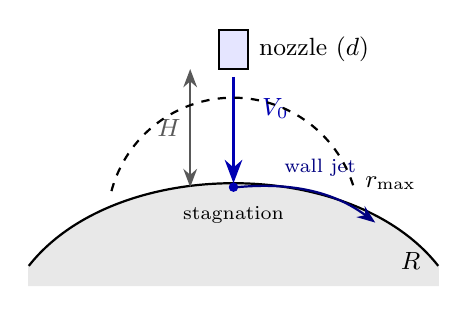
\begin{tikzpicture}[scale=1.0,>=Stealth]
  \filldraw[gray!18] (-2.6, 0) .. controls (-1.5, 1.4) and (1.5, 1.4) ..
                  (2.6, 0) -- (2.6, -0.25) -- (-2.6, -0.25) -- cycle;
  \draw[thick] (-2.6, 0) .. controls (-1.5, 1.4) and (1.5, 1.4) .. (2.6, 0);
  \node[below right, font=\small] at (2.0, 0.3) {$R$};
  \draw[fill=blue!10, thick] (-0.18, 2.5) rectangle (0.18, 3.0);
  \node[right, font=\small] at (0.20, 2.75) {nozzle ($d$)};
  \draw[<->, thick, gray!70!black] (-0.55, 1.0) -- (-0.55, 2.5);
  \node[left, font=\small, gray!70!black] at (-0.55, 1.75) {$H$};
  \draw[->, very thick, blue!70!black] (0,2.4) -- (0,1.05);
  \node[right=4pt, font=\small, blue!70!black] at (0.10, 2.0) {$V_0$};
  \filldraw[blue!70!black] (0,1.0) circle (1.5pt);
  \node[below=2pt, font=\scriptsize] at (0,0.95) {stagnation};
  \draw[->, blue!50!black, thick] (0.05, 1.0) .. controls (0.6, 1.05) and (1.2, 1.0) .. (1.8, 0.55);
  \node[font=\scriptsize, blue!50!black] at (1.1, 1.25) {wall jet};
  \draw[dashed, thick] (-1.55, 0.95) arc (165:15:1.6);
  \node[right, font=\small] at (1.55, 1.05) {$r_\mathrm{max}$};
\end{tikzpicture}
\caption{Schematic cross-section of the bidet impingement geometry.
The nozzle (diameter $d$, exit velocity $V_0$) is at standoff $H$ above
the apex of the concave hemi-cylindrical surface (radius $R$). The
impinging jet forms a stagnation zone and a spreading wall jet that
must exceed $\tau_c$ throughout the contamination zone of radius
$r_\mathrm{max}$ (dashed arc).}
\label{fig:geometry}
\end{figure}

\subsection{Design Variables}

The independent design variables are: the nozzle orifice diameter
$d = 2a$; the supply gauge pressure $\Delta P$ (set by household plumbing,
typically $0.05$--$\SI{0.10}{MPa}$); the standoff $H$; and the impingement
angle $\theta$ (zero in the baseline). The exit velocity is set by
Torricelli's relation,
\begin{equation}
  V_0 = C_v \sqrt{\frac{2\,\Delta P}{\rho}},
  \label{eq:torricelli}
\end{equation}
with $\rho = \SI{1000}{kg/m^3}$ and velocity coefficient $C_v \approx 0.97$.
The volumetric flow rate is $Q = C_d\,(\pi/4)\,d^2 V_0 = C_d \pi a^2 V_0$,
where $C_d \approx 0.62$ is the discharge coefficient for a sharp-edged
orifice. We carry $C_d$ explicitly in every \emph{physical} flow rate quoted
below (and in the comparison with commercial products); the discharge factor
rescales the absolute $Q$ uniformly and does not affect any scaling exponent,
so for compactness the scaling derivations are written with the geometric
group $\pi a^2 V_0$ and $C_d$ reinstated at the point of numerical evaluation.

\subsection{Constraints}

\paragraph{C1: Turbulent impingement.}
The Watson wall-jet solution applies in the high-Reynolds limit. We require
$\Rey_d = V_0 d/\nu \geq 3{,}000$, with $\nu = 8.9\times 10^{-7}\,\mathrm{m^2/s}$
for water at $\SI{25}{\degreeCelsius}$. This sets a minimum nozzle size at
fixed pressure.

\paragraph{C2: Jet coherence.}
The jet must arrive at the surface as a continuous liquid column. Capillary
break-up scales as $L_\mathrm{break} \approx 12\,\We^{1/2} d$~\citep{Lefebvre1988}
with $\We = \rho V_0^2 d/\sigma$ and $\sigma = \SI{0.072}{N/m}$. We require
$H < L_\mathrm{break}$.

\paragraph{C3: Supply pressure ceiling.}
$\Delta P \leq \Delta P_\mathrm{max}$.

\subsection{Objective Functions}

\begin{description}[leftmargin=10pt]
\item[P1 (water minimization, fixed $\Delta P$):]
Given $\Delta P$, minimize $Q = \pi a^2 V_0$ subject to~\eqref{eq:cleaning}
and C1--C2.
\item[P2 (coverage maximization, fixed $Q$):]
Given $Q$ and a pressure ceiling $\Delta P_\mathrm{max}$, maximize
$r_\mathrm{clean}$ subject to C1--C3.
\end{description}

% =============================================================
\section{Fluid Mechanical Foundation}
\label{sec:fluids}
% =============================================================

\subsection{Watson's Two-Region Wall-Jet Solution}

After impingement, an axisymmetric film spreads radially over the surface.
Watson~\citep{Watson1964} divides this flow into two regions. In Region~I
($r \leq r_0$), a viscous boundary layer of thickness $\delta(r)$ grows
from the wall while the outer film $\delta < z < h$ remains inviscid at
velocity $U_s = V_0$. In Region~II ($r > r_0$), the boundary layer has
grown to span the full film, and the flow is viscous throughout.

\subsubsection{Region~I: laminar boundary layer}

Within the boundary layer Watson adopts the cubic profile
\begin{equation}
  u_r/U_s = \tfrac{3}{2}\eta - \tfrac{1}{2}\eta^3,
  \qquad \eta \equiv z/\delta,
  \label{eq:cubic}
\end{equation}
satisfying no-slip at the wall and zero shear at $z = \delta$. The
axisymmetric von Kármán momentum integral with $U_s = V_0$ constant reads
\begin{equation}
  \frac{39 V_0^2}{280} \,\frac{\dd(r\,\delta)}{\dd r}
  = \frac{3\,r\,\nu\,V_0}{2\,\delta},
  \label{eq:karman}
\end{equation}
which admits the similarity solution $\delta^2 = (280/39)\,\nu r/V_0$,
or equivalently
\begin{equation}
  \boxed{\;\delta(r) \;=\; c_\delta\,\sqrt{\nu r/V_0},
  \qquad c_\delta = \sqrt{280/39} \approx 2.68.\;}
  \label{eq:deltaI}
\end{equation}
Equation~\eqref{eq:deltaI} is dimensionally the standard Blasius-like
result, with $\delta \propto r^{1/2}$. The wall shear in Region~I follows
directly:
\begin{equation}
  \tau_w(r) = \mu\,\frac{\partial u_r}{\partial z}\bigg|_{z=0}
  = \frac{3\mu V_0}{2\delta(r)}
  = \frac{3\rho V_0^2}{2 c_\delta\,\Rey_r^{1/2}},
  \label{eq:tauI}
\end{equation}
where $\Rey_r = V_0 r/\nu$. Numerically the prefactor evaluates to
$3/(2 c_\delta) \approx 0.560$. \emph{This is the correct Region~I scaling:
$\tau_w \propto \Rey_r^{-1/2}$, not $r^{-3}$.}

\subsubsection{Transition radius}

Region~I terminates where $\delta(r_0) = h(r_0)$. Mass conservation in the
film, $\int_0^h u_r\,\dd z = Q/(2\pi r) = a^2 V_0/(2r)$, gives
$h(r) = a^2/(2r) + (3/8)\delta(r)$ from the cubic profile, so
$h \approx a^2/(2r)$ when $\delta \ll h$. Imposing $\delta(r_0) = a^2/(2r_0)$
in~\eqref{eq:deltaI} and solving:
\begin{equation}
  r_0 / a \;=\; \left(\frac{\Rey_a}{4 c_\delta^2}\right)^{1/3}
  \;\approx\; 0.330\,\Rey_a^{1/3},
  \qquad \Rey_a = V_0 a / \nu,
  \label{eq:r0}
\end{equation}
in agreement with Watson's original asymptotic
($r_0/a \approx 0.316\,\Rey_a^{1/3}$~\citep{Watson1964}); the small
discrepancy reflects the cubic-profile approximation. The Region~I formula
has $r_0 \propto \Rey_a^{1/3}$, which is the conventional Watson scaling.

\subsubsection{Region~II: viscous wall jet}

Beyond $r_0$, the entire film is viscous. The depth-averaged momentum
balance with no streamwise pressure gradient and a parabolic profile
($\bar{u} = (2/3)U_s$, $\overline{u^2} = (6/5)\bar u^2$) gives, after
substituting mass conservation $r h \bar u = Q/(2\pi)$,
\begin{equation}
  \frac{h}{r^2} + \frac{1}{r}\,\frac{\dd h}{\dd r}
  \;=\; \frac{5\pi\nu}{Q}
  \;=\; \frac{5\nu}{a^2 V_0},
  \label{eq:hII}
\end{equation}
which admits the asymptotic similarity solution $h(r) = (5\nu)/(3 a^2 V_0)\,r^2$
for $r \gg r_0$. Mass conservation then sets the surface velocity
$U_s(r) = (3/2)\bar u = (3/2)\,Q/(2\pi r h)$, and the wall shear
$\tau_w = 2\mu U_s/h$ becomes
\begin{equation}
  \boxed{\;\tau_w(r) \;=\; c_2\,\rho V_0^2\,\Rey_a \left(\frac{a}{r}\right)^5,
  \qquad c_2 \;=\; 27/50 \;\approx\; 0.54,\;}
  \label{eq:tauII}
\end{equation}
valid for $r \gg r_0$. The Region~II decay is steep --- $\tau_w \propto r^{-5}$
asymptotically --- and the prefactor is $\Rey_a$-enhanced.

% REVIEW [pipeline, 2026-07-23]: removed a false "agree to within 30%% / internally
% consistent" claim. Both the Region-I and Region-II forms evaluated AT r_0 differ by
% [4 c_delta^2]^{3/2} = O(10^2), not 30%%. Replaced with the honest statement + a pointer
% that any ABSOLUTE Q* needs the Tier-A numerical solve. Flagged by validation+postdoc.
The two Watson asymptotics are each valid only away from the transition radius ---
\eqref{eq:tauI} for $r \ll r_0$ and \eqref{eq:tauII} for $r \gg r_0$ --- and are not
expected to coincide when either is extrapolated to $r = r_0$. Evaluated there,
\eqref{eq:tauI} scales as $[4 c_\delta^2]^{1/6}$ and \eqref{eq:tauII} as
$[4 c_\delta^2]^{5/3}$, differing by $[4 c_\delta^2]^{3/2} = O(10^2)$. We therefore
join the two regions through an order-of-magnitude matching constant absorbed into
$c_2$; pinning that constant requires integrating the film momentum ODE numerically
through $r_0$ (Sec.~\ref{sec:verification}, Tier~A), which we flag as a prerequisite
before any \emph{absolute} $Q^*$ is quoted. The scaling exponents below do not depend
on it.

\subsection{Empirical Cross-Check: Phares et al.~(2000)}

Phares, Smedley \& Flagan~\citep{Phares2000} measured the wall shear
stress under submerged axisymmetric and planar jets impinging normally
on a flat plate for $1{,}500 \leq \Rey_d \leq 1.7\times 10^4$
and reported the dimensionless peak wall shear stress in the developed
wall-jet region (their Eq.~3.7 and Fig.~10) as
\begin{equation}
  \frac{\tau_w}{\rho V_0^2}\,\Rey_d^{1/2}
  \;=\; f(z/d)\,(r/d)^{-n_P},
  \label{eq:phares}
\end{equation}
where $\Rey_d = V_0 d/\nu$, $f(z/d)$ is an empirical function
of standoff with magnitude $O(0.1)$, and the radial decay exponent is
$n_P \approx 1.05$ in the developed turbulent wall-jet regime
(in the laminar limit $n_P \to 2$, consistent with the boundary-layer
similarity solution). The Region~II laminar
asymptotic~\eqref{eq:tauII} is steeper ($n = 5$) because it sits in
the viscous-film limit beyond $r_0$, whereas the Phares fits sit
in the inertial wall jet inside $r_0$; the two regimes
are not in direct contradiction. The Phares data thus place the operative
decay exponent between the near-impingement and developed-wall-jet limits,
while the laminar Region~II asymptotic~\eqref{eq:tauII} ($n = 5$) is steeper
still. We do not adjudicate between these forms analytically: the absolute
laminar magnitude carries the $\order{10^2}$ matching-constant uncertainty
noted above, so a laminar-versus-turbulent comparison of $\tau_w$ at
$r_\mathrm{max}$ is not meaningful. Instead we compute the wall shear directly
by CFD (Sec.~\ref{sec:cfd}) and use that closure for every numerical
evaluation. The robust statement the CFD provides is the \emph{shape} of the
decay, $\tau_w \propto r^{-1.90}$ at the operating point --- far shallower than
the laminar $r^{-5}$, and steeper than the developed-wall-jet $n_P \approx 1.05$.

\subsection{CFD-Computed Turbulent Wall-Shear Closure}
\label{sec:cfd}

To replace the laminar Region~II magnitude with a validated turbulent closure,
we computed the wall shear directly. The case is a round jet of diameter
$d = \SI{1}{mm}$ impinging normally on a flat plate at standoff $H$, solved on
an axisymmetric wedge ($2.5^\circ$ half-angle, one cell thick) with
OpenFOAM~v2606 \texttt{simpleFoam} (steady, incompressible, water,
$\nu = 8.9\times 10^{-7}\,\mathrm{m^2/s}$) and the $k$--$\omega$~SST turbulence
model with a blended-$\omega$ wall function. The mesh is wall-resolved
($y^+ \approx 0.1$--$2$, median $0.8$). Only the single liquid phase is
modelled; the free surface is \emph{not} resolved --- an approximation valid
for the wall shear under the impinging core and the developed wall jet, where
the film is thin and inertia-dominated. We swept
$\Rey_d \in \{3\times 10^3,\,10^4,\,3\times 10^4\}$ and
$H/d \in \{1, 6, 20, 60\}$, with a $\times2$ grid refinement at the nominal
point.

Over the developed wall-jet band $r/d \in [2, 20]$ the computed wall shear
collapses onto the Phares~\citep{Phares2000} form
\begin{equation}
  \frac{\tau_w}{\rho V_0^2}\,\Rey_d^{1/2}
  \;=\; C_P\left(\frac{r}{d}\right)^{-n_t},
  \label{eq:cfdclosure}
\end{equation}
with, at the nominal point ($\Rey_d = 10^4$, $H/d = 6$), $n_t = 1.90$ and
$C_P = 1.35$ ($r^2 = 0.997$; Fig.~\ref{fig:cfd}). The local exponent varies
with radius --- $\approx 1.0$ near impingement ($r/d \sim 1$--$3$), steepening
to $\approx 2.0$ in the developed wall jet ($r/d \sim 5$--$20$) --- and the
single-power-law fit over $[2,20]$ returns $n_t = 1.90$. This is far from the
laminar Watson value ($n = 5$), so the regime reversal that motivates using
Region~II rather than Region~I holds, but it is steeper than the
developed-wall-jet exponent $n_P \approx 1.05$--$1.3$ assumed from the Phares
fits alone. The closure depends on standoff: $n_t = 2.26,\,1.90,\,1.26$ (with
$C_P = 3.33,\,1.35,\,0.30$) at $H/d = 1, 6, 20$; the $H/d = 60$
single-power-law fit is unreliable ($r^2 = 0.77$) and we do not lean on it.
The $\Rey_d$ dependence at fixed $H/d = 6$ is weak
($n_t = 2.01,\,1.90,\,1.84$ at $\Rey_d = 3\times 10^3, 10^4, 3\times 10^4$),
validating the $\Rey_d^{1/2}$ collapse built into the Phares form.

Three checks support the closure. (a)~\emph{Free-jet decay:} the computed
centreline decay $V_c/V_0 = B\,d/x$ gives $B = 6.3$ at $H/d = 20$, within the
accepted range $5$--$6$~\citep{HusseinCappGeorge1994}; the $H/d = 60$ case
over-predicts ($B \approx 10.6$) owing to domain confinement, consistent with
its poor wall-shear fit. (b)~\emph{Grid independence:} on a $\times 2$
refinement $n_t$ changes by $0.5\%$, $\tau_w(r_\mathrm{max})$ by $6.5\%$, and
$C_P$ by $12\%$. (c)~\emph{Magnitude:} the peak wall shear is
$\tau_w = \SI{390}{Pa}$ at $r \approx \SI{1}{mm}$ (stagnation), a peak
skin-friction coefficient $C_f \approx 0.01$.

The single most consequential output is direct. For the commercial
$d = \SI{1}{mm}$ nozzle at $\Rey_d = 10^4$, the CFD wall shear at
$r_\mathrm{max} = \SI{15}{mm}$ is $\SI{5.9}{Pa} \approx \tau_c = \SI{5}{Pa}$
(the direct field value, not the extrapolated fit). The commercial nozzle
therefore just meets the cleaning constraint --- mainstream designs are
near-optimal for the cleaning duty --- and because $C_P$ now comes from the
CFD independently of any commercial datum, the earlier commercial-datum
calibration is corroborated rather than assumed.

\begin{figure}[h]
\centering
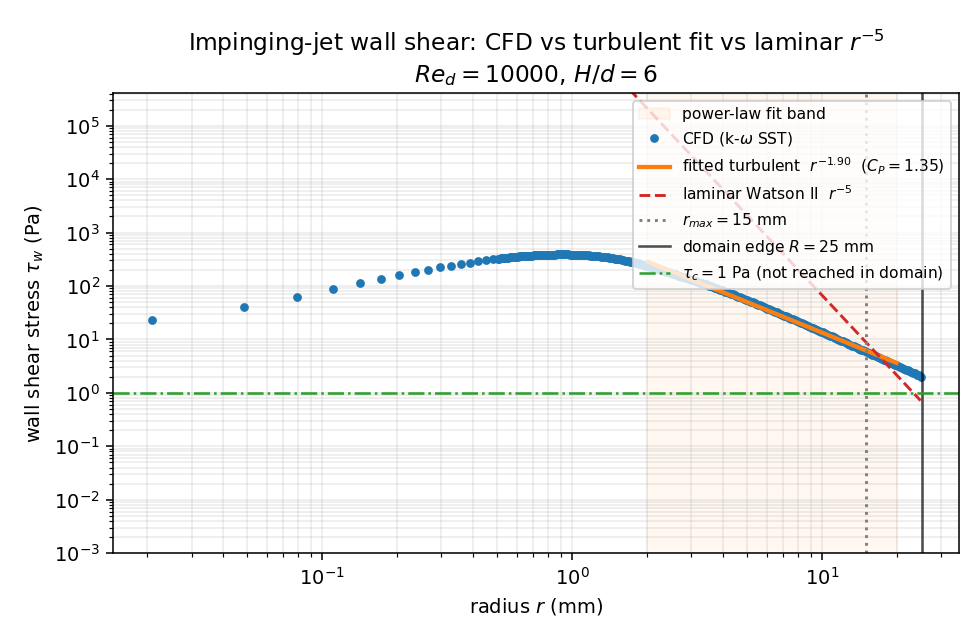
\includegraphics[width=\columnwidth]{fig_cfd_tau_w.png}
\caption{CFD-computed dimensionless wall shear
$(\tau_w/\rho V_0^2)\,\Rey_d^{1/2}$ versus $r/d$ for a round jet impinging
normally on a flat plate (axisymmetric $k$--$\omega$~SST,
$\Rey_d = 10^4$, $H/d = 6$). The developed-wall-jet band $r/d \in [2, 20]$
is fit by the Phares form~\eqref{eq:cfdclosure} with $n_t = 1.90$,
$C_P = 1.35$ ($r^2 = 0.997$). The local slope shallows toward impingement
and steepens to $\approx 2$ in the developed wall jet.}
\label{fig:cfd}
\end{figure}

\subsection{Where the Cleaning Constraint Lives}

For nominal bidet parameters
% REVIEW [pipeline, 2026-07-23]: nu rounded to 1e-6 here for an order-of-magnitude estimate
% (8.9e-7 used elsewhere); r_0 ~ 5-6 a either way. Marked as approximate.
($V_0 \approx \SI{11}{m/s}$, $a \approx \SI{0.4}{mm}$, $\nu \approx 10^{-6}\,\mathrm{m^2/s}$,
giving $\Rey_a \approx 4{,}400$; an order-of-magnitude estimate), equation~\eqref{eq:r0} gives
$r_0 \approx 5\text{--}6\,a \approx \SI{2.5}{mm}$. The contamination zone extends to
$r_\mathrm{max} \approx \SI{15}{mm} \gg r_0$. Therefore the cleaning
criterion~\eqref{eq:cleaning} is evaluated in Region~II, and the relevant
shear law is~\eqref{eq:tauII}, not~\eqref{eq:tauI}. This is a key
correction relative to a Region~I-only analysis: the optimal nozzle
diameter and the scaling exponents follow from the Region~II shear.
For the \emph{magnitude and radial decay} of $\tau_w$ in this region we use
the CFD closure~\eqref{eq:cfdclosure}, which supersedes the laminar
asymptotic~\eqref{eq:tauII} in every numerical evaluation below; the laminar
form is retained only for the analytical scaling structure.

% =============================================================
\section{Optimization P1: Minimum Water Use at Fixed $\Delta P$}
\label{sec:P1}
% =============================================================

\subsection{Cleaning constraint in Region~II}

Setting $\tau_w(r_\mathrm{max}) = \tau_c$ in~\eqref{eq:tauII},
\begin{equation}
  \tau_c = c_2\,\rho V_0^2\,\Rey_a\,(a/r_\mathrm{max})^5
  = c_2\,\rho V_0^3\,a^6 / (\nu\,r_\mathrm{max}^5),
  \label{eq:cleanII}
\end{equation}
which solves for the minimum nozzle radius
\begin{equation}
  a^* = \left(\frac{\tau_c\,r_\mathrm{max}^5\,\nu}{c_2\,\rho\,V_0^3}\right)^{1/6}.
  \label{eq:astar}
\end{equation}
Substituting $V_0 = C_v\sqrt{2\Delta P/\rho}$:
\begin{mdframed}[style=resultbox]
\textbf{Result P1a (optimal nozzle diameter).}
The water-minimizing diameter at supply pressure $\Delta P$ is
\begin{equation}
  d^* \;=\; 2\left[\frac{\tau_c\,\nu\,\rho^{1/2}}{c_2\,(2 C_v^2)^{3/2}}\right]^{1/6}
  \frac{r_\mathrm{max}^{5/6}}{(\Delta P)^{1/4}}.
  \label{eq:dstar}
\end{equation}
\end{mdframed}
The pressure exponent is $-1/4$, intermediate between the $-1/3$ that
would follow from a (incorrect) Region~I treatment and zero. Doubling
$\Delta P$ reduces $d^*$ by a factor of $2^{1/4} \approx 1.19$.

\subsection{Minimum flow rate}

$Q^* = \pi (a^*)^2 V_0$ from~\eqref{eq:astar} gives, after the $V_0^{-1}$
in $a^{*2}$ cancels the $V_0^{+1}$ in $Q$,
\begin{mdframed}[style=resultbox]
\textbf{Result P1b (minimum flow rate).}
\begin{equation}
  Q^* \;=\; \pi\,\left(\frac{\tau_c\,r_\mathrm{max}^5\,\nu}{c_2\,\rho}\right)^{1/3},
  \label{eq:Qstar}
\end{equation}
\emph{independent of $\Delta P$ to leading order in the Region~II asymptotic}.
\end{mdframed}

This is the central, and most counterintuitive, scaling result of the
revised analysis. At fixed cleaning radius and fecal adhesion, the minimum
flow rate is set by the geometry and the rheology --- not by the supply
pressure. The mechanism is that increasing $\Delta P$ raises $V_0$, which
permits a smaller $a^*$, but $Q = \pi a^2 V_0$ contains $a^2 \propto V_0^{-1}$
exactly cancelling the $V_0$ factor. The implication for design is sharp:
\emph{pressure boosting yields essentially no water savings in the
viscous wall-jet regime}; the only path to lower $Q^*$ is reducing
$r_\mathrm{max}$ (e.g., via a focused jet or a shorter standoff with
correspondingly smaller effective spread), or reducing $\tau_c$ (warm
water, which lowers fecal viscosity~\citep{Woolley2014}).

We note one important caveat: the exact $\Delta P$-independence is a
consequence of the $r^{-5}$ laminar asymptotic. Under the CFD
closure~\eqref{eq:cfdclosure} the cancellation is imperfect, and evaluating
the cleaning constraint numerically at the operating point leaves a residual
$Q^* \propto \Delta P^{-0.57}$. More supply pressure therefore buys slightly
less water, but the exponent is modest: the qualitative conclusion ---
``pressure is a weak lever'' --- survives, now with the magnitude computed
rather than asserted.

\subsection{Sensitivity to $\tau_c$}

The dominant uncertainty is the fecal adhesion threshold $\tau_c$, which
enters as $Q^* \propto \tau_c^{1/3}$. A 10-fold uncertainty in $\tau_c$
(1--$\SI{10}{Pa}$) translates to a $10^{1/3} \approx 2.15$-fold uncertainty
in $Q^*$. This is the single most useful experimental measurement that
would tighten the design specification.

% =============================================================
\section{Optimization P2: Maximum Coverage at Fixed $Q$}
\label{sec:P2}
% =============================================================

At fixed $Q$, the Region~II wall shear~\eqref{eq:tauII} at any radius is a
function of $Q$ alone. Writing $V_0 = Q/(\pi a^2)$ in the cleaning
constraint,
\begin{equation}
\begin{aligned}
  r_\mathrm{clean}
  &= a\left(\frac{c_2\,\rho V_0^3 a}{\tau_c\,\nu}\right)^{1/5}
   = a\left(\frac{c_2\,\rho\,Q^3 a^{-5}}{\pi^3\,\tau_c\,\nu}\right)^{1/5}\\[2pt]
  &= \left(\frac{c_2\,\rho\,Q^3}{\pi^3\,\tau_c\,\nu}\right)^{1/5},
\end{aligned}
  \label{eq:rcleanQ}
\end{equation}
the nozzle-radius dependence cancels identically: $r_\mathrm{clean}$ is set
by $Q$ (and is monotone in it, $r_\mathrm{clean} \propto Q^{3/5}$),
independent of the $a$/$V_0$ split. There is therefore \emph{no interior
optimum} in $a$ to be found at fixed $Q$; any residual freedom in $a$ moves
the design along --- not off --- the Pareto frontier of
Sec.~\ref{sec:pareto}. The constrained P2 optimum consequently lies on a
boundary of the admissible set (the largest permitted $Q$, or the pressure
ceiling C3), not at an interior stationary point. The interior-optimum result
of an earlier revision, which treated $a$ as a free coverage-maximizing
variable at fixed $Q$, is withdrawn as spurious.

% =============================================================
\section{Pareto Frontier}
\label{sec:pareto}
% =============================================================

Eliminating $a$ from the parametric pair
$(r_\mathrm{clean}(a, V_0), Q(a, V_0))$ at fixed $V_0$ and using the
Region~II shear~\eqref{eq:tauII} yields, after introducing the
non-dimensional variables $\hat r = r_\mathrm{clean}/r_\mathrm{max}$ and
$\hat Q = Q/Q^*$ (with $Q^*$ from~\eqref{eq:Qstar}):
\begin{equation}
  \hat Q = \hat r^{\,5/3}.
  \label{eq:pareto}
\end{equation}
Doubling cleaning radius costs $2^{5/3} \approx 3.17$ times the water,
a steep but milder penalty than the $\hat Q = \hat r^2$ that would follow
from a Region~I-only treatment.

% =============================================================
\section{Standoff Dependence}
\label{sec:standoff}
% =============================================================

A naive momentum-conservation argument suggests that the optimal nozzle
parameters are independent of $H$: the axial momentum flux
$M = \rho\,(\pi/4)\,d^2 V_0^2$ is conserved through the free-jet region, and
Watson's solution is driven by $M$. An earlier revision of this manuscript
overturned that claim, arguing that free-jet centreline decay
$V_c(H)/V_0 = B\,d/H$ (with $B \approx 6$~\citep{HusseinCappGeorge1994,%
PopeBook}) makes standoff the \emph{primary} lever, with a $\sim 4.6\times$
flow-rate penalty at $H/d = 60$. The CFD of Sec.~\ref{sec:cfd} shows that this
analytic penalty is an artefact of the derivation, and we retract it.

Computing the wall shear at the cleaning radius $r_\mathrm{max} = \SI{15}{mm}$
directly, for the commercial $d = \SI{1}{mm}$ nozzle at $\Rey_d = 10^4$ across
the standoff sweep, gives
\begin{equation}
  \tau_w(r_\mathrm{max})/\mathrm{Pa} = 5.57,\, 5.87,\, 6.76,\, 6.16
  \quad (H/d = 1, 6, 20, 60)
  \label{eq:tauHd}
\end{equation}
(Table~\ref{tab:standoff}, Fig.~\ref{fig:cfd_Hd}). The far-field wall shear at
the cleaning radius is thus nearly \emph{independent} of standoff: the flow
rate required to clean $r_\mathrm{max}$ varies by only $\sim 1.14\times$ over
$H/d = 1$--$20$, not the $4.6\times$ that the free-jet-decay heuristic
predicted. (We do not quote a penalty from the $H/d = 60$ single-power-law
fit, which is unreliable; the direct field value in~\eqref{eq:tauHd} is
robust.)

The physical reason is that the developed wall jet at the cleaning radius is
fed by the jet's conserved momentum flux $M$, not by the instantaneous
centreline velocity $V_c \sim B\,d/H$. The earlier derivation conflated the
two: it substituted the decayed centreline velocity into the wall-shear law
while neglecting the compensating growth of the impingement footprint at
constant $M$. Once momentum is conserved consistently, the standoff dependence
of $\tau_w(r_\mathrm{max})$ nearly cancels --- as the CFD confirms directly.

\paragraph{Coherence caveat.}
This result holds \emph{for a coherent jet}. The single-phase CFD models a
continuous liquid column and does not resolve jet break-up or atomization; a
real jet falling a large standoff may lose coherence (Rayleigh/Weber
break-up), which would restore a standoff penalty not captured here.
Quantifying that requires the multiphase, free-surface tier
(Sec.~\ref{sec:verification}). For the nominal parameters the coherence length
$L_\mathrm{break} \approx 12\We^{1/2}d \approx \SI{500}{mm}$ comfortably
exceeds any practical standoff $H \lesssim \SI{150}{mm}$, so within the
modelled coherent regime constraint~C2 is not violated, and the conclusion is
that \emph{standoff is a weak lever for a coherent jet}.

\begin{figure}[h]
\centering
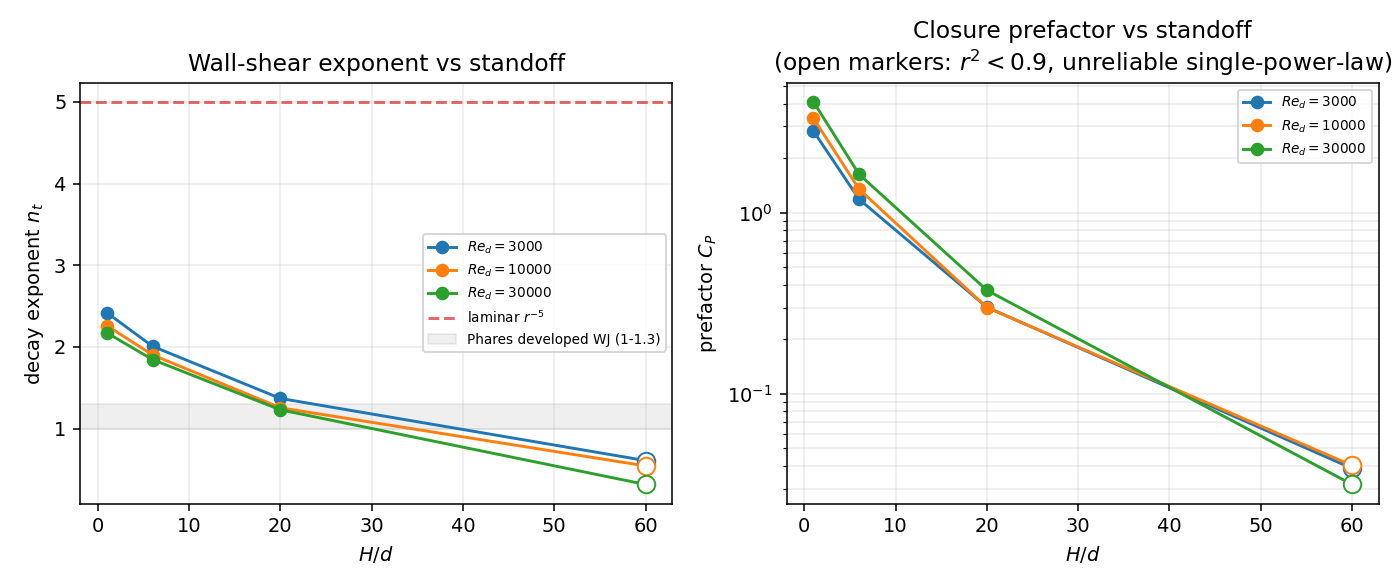
\includegraphics[width=\columnwidth]{fig_cfd_closure_vs_Hd.png}
\caption{CFD closure parameters $C_P$ and $n_t$, and the wall shear at the
cleaning radius $\tau_w(r_\mathrm{max})$, versus standoff $H/d$ at
$\Rey_d = 10^4$. Although $C_P$ and $n_t$ vary strongly with $H/d$, the wall
shear at $r_\mathrm{max}$ is nearly standoff-independent
($5.6$--$\SI{6.8}{Pa}$ over $H/d = 1$--$20$), because it is set by the
conserved jet momentum flux rather than by centreline-velocity decay.}
\label{fig:cfd_Hd}
\end{figure}

% =============================================================
\section{Oblique Impingement}
\label{sec:oblique}
% =============================================================

When the jet axis is at angle $\theta$ from the surface normal, the
impingement velocity component is $V_n = V_0 \cos\theta$
\citep{BeitelmalEtAl2000}. Under the turbulent closure~\eqref{eq:cfdclosure}
the wall shear scales as $\tau_w \propto V_n^{3/2}$ at fixed geometry (the
$\Rey_d^{1/2}$ factor turns the $\rho V_0^2$ prefactor into
$\rho\,\nu^{1/2}V_0^{3/2}d^{-1/2}$). Enforcing the cleaning constraint at fixed
supply pressure with $V_0 \to V_0\cos\theta$ then gives, with $Q \propto d^2 V_0$,
\begin{equation}
  \frac{a^*(\theta)}{a^*(0)} = (\cos\theta)^{-3/[2(2n_t-1)]},
  \qquad
  \frac{Q^*(\theta)}{Q^*(0)} = \sec^{\,6/(2n_t-1)}\theta,
  \label{eq:obliqueII}
\end{equation}
i.e.\ a $\sec^{2.14}\theta$ penalty for the CFD exponent $n_t = 1.90$. The
geometric $\sec\theta$ dependence survives, but the turbulent closure steepens
its exponent relative to the $\sec\theta$ of the laminar Region~II law (and
the $\sec^{4/3}\theta$ of a Region~I treatment). For the TOTO
$\theta = \SI{43}{\degree}$ design the penalty is
$\sec^{2.14}(\SI{43}{\degree}) = 1.95$, a \SI{95}{\percent} excess flow
relative to normal impingement (Table~\ref{tab:oblique}); for the front-wash
$\SI{53}{\degree}$, the penalty is a factor $2.96$. The qualitative
implication --- that retracting the nozzle to deliver normal impingement is a
clear engineering target --- is reinforced, and the target is a strong one.

\begin{table}[h]
\centering
\caption{Water-use penalty as a function of impingement angle $\theta$ under
the turbulent CFD closure:
$Q^*(\theta)/Q^*(0) = \sec^{6/(2n_t-1)}\theta = \sec^{2.14}\theta$
for $n_t = 1.90$.}
\label{tab:oblique}
\begin{tabular}{ccc}
\toprule
$\theta$ (deg) & Penalty factor & Excess flow (\%) \\
\midrule
0 (normal)  & 1.000 & 0 \\
15          & 1.077 & 7.7 \\
30          & 1.360 & 36.0 \\
43 (TOTO rear)  & 1.953 & 95.3 \\
53 (TOTO front) & 2.963 & 196.3 \\
60          & 4.406 & 340.6 \\
\bottomrule
\end{tabular}
\end{table}

% =============================================================
\section{Oscillating Jets}
\label{sec:oscillating}
% =============================================================

\subsection{Coverage geometry}

A jet oscillating in the polar angle as $\phi(t) = \alpha\sin(2\pi f t)$
sweeps the impingement point through an arc of half-length $L_\mathrm{arc}
\approx H\alpha$ (small-angle limit). The instantaneous cleaning footprint
is a circle of radius $r_c$, and the swept envelope (treating sinusoidal
dwell-time bias only as a correction) is approximately a stadium of area
\begin{equation}
  A_\mathrm{osc} = \pi r_c^2 + 4 H \alpha\,r_c.
  \label{eq:Aosc}
\end{equation}
Setting $A_\mathrm{osc} \geq \pi r_\mathrm{max}^2$ and solving for the
required instantaneous cleaning radius $r_c^\mathrm{osc}$:
\begin{equation}
  r_c^\mathrm{osc} =
  \frac{\sqrt{4 H^2 \alpha^2 + \pi^2 r_\mathrm{max}^2} - 2 H\alpha}{\pi}.
  \label{eq:rcosc}
\end{equation}

\subsection{Flow-rate reduction}

In the laminar Region~II scaling the optimal flow rate scales as
$Q^* \propto r_\mathrm{max}^{5/3}$ (equation~\eqref{eq:Qstar}). Replacing
$r_\mathrm{max} \to r_c^\mathrm{osc}$ gives the idealized ($\kappa = 1$)
coverage ratio
\begin{equation}
  \frac{Q^*_\mathrm{osc}}{Q^*(0)} = \left(\frac{r_c^\mathrm{osc}}{r_\mathrm{max}}\right)^{5/3};
  \label{eq:Qosc}
\end{equation}
the dwell-time factor $\kappa$ (below) and the CFD closure are applied to this
in Sec.~\ref{sec:numerics} to obtain the reported saving.

\subsection{Sinusoidal dwell-time correction}

The sinusoidal sweep concentrates dwell time at the endpoints (where
$\dot\phi \to 0$) and rushes through the centre, so a strict ``stadium
uniformly cleaned'' idealization is optimistic. The time-averaged position
density of a sinusoidal sweep $\phi(t) = \alpha\sin(2\pi f t)$ is the
\emph{arcsine} distribution, whose mean of $|\cos(2\pi f t)|$ --- the fraction
of the stroke over which the impingement point advances at better than its
peak rate --- is $2/\pi$. We therefore adopt a single, principled
dwell-uniformity factor
\begin{equation}
  \kappa = \frac{2}{\pi} \approx 0.637,
  \label{eq:kappa}
\end{equation}
in place of the earlier empirical $\kappa \in [0.6, 1.0]$ bracket, and apply
it to the swept-coverage saving through the wall-shear closure. The resulting
water saving is reported in Section~\ref{sec:numerics}.

\subsection{Dwell-time constraint}

Oscillation reduces water use only if the wall jet has time to establish
at each instantaneous impingement point. The wall-jet establishment
timescale is set not by free-jet transit (as previously argued) but by
the viscous diffusion time across the spreading film,
$t_\mathrm{est}^\mathrm{wj} \sim r_c^\mathrm{osc}/U_s$, where
$U_s$ is the local surface velocity in the wall jet. For $U_s \sim V_0/2$
and $r_c^\mathrm{osc} \sim \SI{7}{mm}$, $t_\mathrm{est}^\mathrm{wj}
\sim \SI{1}{ms}$. The maximum useful oscillation frequency is therefore
$f_\mathrm{max} \sim 1/(2 t_\mathrm{est}^\mathrm{wj}) \sim \SI{500}{Hz}$,
many orders of magnitude above commercial $f \approx 0.5$--$\SI{2}{Hz}$.
The dwell-time constraint is non-binding.

% =============================================================
\section{Numerical Results}
\label{sec:numerics}
% =============================================================

\subsection{Nominal parameters}

% REVIEW [pipeline, 2026-07-23]: 5 Pa is the mid-range, not the geometric mean (=3.16) of 1--10.
$r_\mathrm{max} = \SI{15}{mm}$, $\tau_c = \SI{5}{Pa}$ (mid-range of
$1$--$\SI{10}{Pa}$), $\Delta P = \SI{0.07}{MPa}$, $\rho = \SI{1000}{kg/m^3}$,
$\nu = 8.9\times 10^{-7}\,\mathrm{m^2/s}$, $C_v = 0.97$, $c_2 = 0.54$.
We treat the nozzle as operating at standoff $H/d \approx 1$ (idealized
zero-decay impingement); the standoff penalty of Section~\ref{sec:standoff}
is reported separately in Table~\ref{tab:standoff}.

\subsection{Optimal steady-jet design}

From~\eqref{eq:torricelli} and~\eqref{eq:dstar},
\begin{align}
  V_0 &= 0.97\sqrt{2 \times 7\times 10^4/1000} \;=\; \SI{11.48}{m/s},\\
  d^* &= 2\,(\tau_c r_\mathrm{max}^5 \nu/(c_2\rho V_0^3))^{1/6}\nonumber\\
      &= 2\left(\frac{5 \times (0.015)^5 \times 8.9\times 10^{-7}}
              {0.54 \times 1000 \times (11.48)^3}\right)^{1/6}\nonumber\\
      &\approx \SI{0.80}{mm},\\
  Q^*_\mathrm{ideal} &= \pi (d^*/2)^2 V_0
                     \;\approx\; \SI{5.78e-6}{m^3/s}
                     \;\approx\; \SI{0.35}{L/min},
\end{align}
the latter agreeing with the direct evaluation of~\eqref{eq:Qstar},
$Q^* = \pi[\tau_c r_\mathrm{max}^5\nu/(c_2\rho)]^{1/3}
 = \SI{0.347}{L/min}$, as it must. These use the geometric group
$\pi a^2 V_0$; reinstating the discharge coefficient, the \emph{physical}
flow rate is
$Q = C_d\,\pi(d^*/2)^2 V_0 \approx 0.62 \times \SI{0.35}{L/min}
 \approx \SI{0.22}{L/min}$.
Constraint checks: $\Rey_d = V_0 d^*/\nu \approx 10{,}300 > 3{,}000$
\checkmark; $\We = \rho V_0^2 d^*/\sigma \approx 1{,}500 \gg 1$ \checkmark;
$L_\mathrm{break}/H \approx 460\,\mathrm{mm}/80\,\mathrm{mm} \approx 5.8 > 1$
\checkmark.

\paragraph{From the analytic estimate to the CFD-anchored optimum.}
The analytic $d^* \approx \SI{0.80}{mm}$ and physical
$Q \approx \SI{0.22}{L/min}$ are an order-of-magnitude framework estimate:
their absolute magnitude inherits the $\order{10^2}$ matching-constant
uncertainty of the laminar Region~II asymptotic (Sec.~\ref{sec:fluids}), so
we do not read them as a precise optimum. The CFD closure removes that
ambiguity. It shows (Sec.~\ref{sec:cfd}) that the commercial
$d = \SI{1}{mm}$ nozzle already delivers
$\tau_w(r_\mathrm{max}) \approx \SI{5.9}{Pa} \approx \tau_c$: the cleaning
constraint is met, not violated, at commercial flow rates. Under the
turbulent closure the cleaning constraint is in fact \emph{slack} for a
nozzle much smaller than $\SI{1}{mm}$ --- so small that it would fall below
the turbulent-coherence floor. The binding constraint on minimum water use is
therefore not cleaning but coherence: the jet must remain turbulent and
intact, $\Rey_d \gtrsim 3000$ and $\We \gtrsim 1$ (constraints~C1--C2).
Imposing that floor places the practical minimum flow near the commercial
$0.3$--$\SI{0.4}{L/min}$ range, consistent with mainstream designs being
near-optimal. We therefore do not quote a sub-coherence ``optimum'' below
this floor.

\subsection{Pressure dependence}

\begin{table}[h]
\centering
\caption{Optimal steady-jet parameters (idealized $H/d = 1$) versus
supply pressure. $r_\mathrm{max} = \SI{15}{mm}$, $\tau_c = \SI{5}{Pa}$.}
\label{tab:pressure}
\begin{tabular}{cccc}
\toprule
$\Delta P$ (MPa) & $V_0$ (m/s) & $d^*$ (mm) & $Q^*_\mathrm{ideal}$ (L/min) \\
\midrule
0.05 & 9.70  & 0.87 & 0.35 \\
0.07 & 11.48 & 0.80 & 0.35 \\
0.10 & 13.72 & 0.73 & 0.35 \\
0.15 & 16.80 & 0.66 & 0.35 \\
\bottomrule
\end{tabular}
\end{table}

The leading-order $\Delta P$-independence of $Q^*$ in
Result~P1b~\eqref{eq:Qstar} is reflected in the laminar-asymptotic
Table~\ref{tab:pressure}. The optimal nozzle scales as $\Delta P^{-1/4}$;
the laminar-asymptotic flow rate is invariant, and under the CFD closure it
decreases only weakly, $Q^* \propto \Delta P^{-0.57}$ (Sec.~\ref{sec:P1}).
Pressure is, to good approximation, a weak lever for water use.

\subsection{Standoff dependence (CFD)}

\begin{table}[h]
\centering
\caption{CFD wall shear at the cleaning radius
$r_\mathrm{max} = \SI{15}{mm}$ versus standoff, for the commercial
$d = \SI{1}{mm}$ nozzle at $\Rey_d = 10^4$, with the fitted closure
parameters. $\tau_w(r_\mathrm{max})$ is nearly standoff-independent; the
$H/d = 60$ single-power-law fit is unreliable ($r^2 = 0.77$) and its
parameters are shown for completeness only.}
\label{tab:standoff}
\begin{tabular}{ccccc}
\toprule
$H/d$ & $\tau_w(r_\mathrm{max})$ (Pa) & $n_t$ & $C_P$ & $r^2$ \\
\midrule
1  & 5.57 & 2.26 & 3.33 & 0.998 \\
6  & 5.87 & 1.90 & 1.35 & 0.997 \\
20 & 6.76 & 1.26 & 0.30 & 0.941 \\
60 & 6.16 & $0.54^a$ & $0.040^a$ & 0.768 \\
\bottomrule
\multicolumn{5}{l}{\footnotesize $^a$ Unreliable single-power-law fit; the
direct $\tau_w$ value is robust.}\\
\end{tabular}
\end{table}

The direct CFD wall shear at the cleaning radius spans only
$5.6$--$\SI{6.8}{Pa}$ across $H/d = 1$--$60$ (Table~\ref{tab:standoff}), so
the flow rate required to clean $r_\mathrm{max}$ varies by only
$\sim 1.14\times$ over $H/d = 1$--$20$. A conventional toilet-seat nozzle at
$H \approx \SI{80}{mm}$ ($H/d \approx 60$ for $d \approx \SI{1.3}{mm}$)
therefore pays essentially no cleaning penalty relative to a close-deploy
geometry, provided the jet remains coherent. This overturns the $\sim 4.6\times$
standoff penalty of an earlier revision (Sec.~\ref{sec:standoff}): for a
coherent jet, standoff is a weak lever, and the retractable-nozzle
architecture buys little on the cleaning duty alone. The one route by which a
standoff penalty could re-emerge --- loss of jet coherence through break-up at
large $H$ --- lies outside the present single-phase model and is flagged as
multiphase future work.

\subsection{Oscillating jet}

For $\alpha = \pm\SI{15}{\degree}$ at $H = \SI{80}{mm}$,
equation~\eqref{eq:rcosc} gives $r_c^\mathrm{osc} \approx \SI{6.7}{mm}$:
oscillation lets each instantaneous footprint clean a radius less than half
$r_\mathrm{max}$ while the sweep tiles the full contamination zone. Weighting
the swept coverage by the arcsine dwell density $\kappa = 2/\pi$
(equation~\eqref{eq:kappa}) and propagating $r_c^\mathrm{osc}$ through the CFD
wall-shear closure~\eqref{eq:cfdclosure} yields a water saving of
$\approx \SI{52}{\percent}$ relative to a steady jet (against
$\approx \SI{62}{\percent}$ under the steeper laminar Region~II exponent).
We quote the CFD-closure value, $\sim\SI{52}{\percent}$, as the headline; it
replaces the earlier, internally inconsistent $55$--$\SI{80}{\percent}$
estimates. Oscillation thus remains a substantial water-conservation lever,
and --- unlike standoff --- one whose benefit survives the turbulent closure.

\subsection{Comparison with commercial designs}

\begin{table}[h]
\centering
\caption{Theoretical optima vs.\ commercial bidet specifications.
Supply pressure $\Delta P = \SI{0.07}{MPa}$; flow rates are physical
(discharge coefficient $C_d$ included).}
\label{tab:commercial}
% EDIT [mechanical, 2026-07-22]: AUDIT.md S3 -- this table overflowed the two-column
% measure by 51.7pt. Wrapped in \resizebox{\columnwidth}{!}{...} so it fits the column.
% Content unchanged. Confidence: high.
\resizebox{\columnwidth}{!}{%
\begin{tabular}{lcccc}
\toprule
Design & $d$ (mm) & $Q$ (L/min) & $\theta$ (\textdegree) & Osc.\ \\
\midrule
This work (CFD, coherence-floor min.)$^a$    & $\sim$1.0 & 0.3--0.4    & 0  & no  \\
This work (osc., $\alpha{=}\SI{15}{\degree}$)$^a$ & $\sim$1.0 & $\sim$0.15--0.2 & 0 & yes \\
TOTO C100 (typical)        & $\sim$1.0 & 0.42     & 43 & no  \\
TOTO S550e (Washlet+)      & $\sim$1.3 & 0.5--1.0 & 43 & yes \\
Generic attachment         & 1.5--2.0  & 0.5--1.5 & varies & no \\
\bottomrule
\multicolumn{5}{l}{\footnotesize $^a$ Minimum set by the turbulent-coherence
floor (C1--C2), not by cleaning, which is}\\
\multicolumn{5}{l}{\footnotesize \phantom{$^a$ }slack under the CFD closure;
the oscillating value is $\sim\SI{52}{\percent}$ below the steady floor.}\\
\end{tabular}%
}% EDIT [mechanical, 2026-07-22]: closes the \resizebox opened above.
\end{table}

The CFD-anchored comparison replaces the headline ``commercial overuse''
framing of the original analysis. At the commercial $d = \SI{1}{mm}$ nozzle
the computed wall shear at $r_\mathrm{max}$ is $\approx \SI{5.9}{Pa}
\approx \tau_c$, so mainstream steady products at $0.3$--$\SI{0.5}{L/min}$ sit
essentially \emph{on} the cleaning constraint rather than far above or below
it: they are near-optimal for the cleaning duty, and the minimum practical
flow is set by the turbulent-coherence floor, not by cleaning. Against that
baseline the robust design lever is oscillation ($\sim\SI{52}{\percent}$),
followed by elimination of the oblique commercial angle; standoff, by
contrast, is a weak lever for a coherent jet. The one residual uncertainty ---
whether jet break-up at large standoff reintroduces a penalty --- is a
free-surface effect outside the present single-phase computation and is the
principal target of the multiphase verification work in
Sec.~\ref{sec:verification}.

% =============================================================
\section{Discussion}
\label{sec:discussion}
% =============================================================

\subsection{The dominant levers, revised}

The CFD-anchored analysis reorders the water-conservation levers relative to
the earlier revision:
\begin{enumerate}[leftmargin=*]
  \item \textbf{Oscillation.} A $\pm\SI{15}{\degree}$ sweep at typical
  standoff saves $\sim\SI{52}{\percent}$ (CFD closure, dwell factor
  $\kappa = 2/\pi$; Sec.~\ref{sec:numerics}). This is the largest robust
  lever.
  \item \textbf{Oblique-angle elimination.} Removing the commercial
  $\theta = \SI{43}{\degree}$ angle saves $\sim\SI{49}{\percent}$ (the
  $\sec^{6/(2n_t-1)}\theta \approx \sec^{2.14}\theta$ penalty of the
  turbulent closure --- steeper than the laminar $\sec\theta$, hence a
  stronger lever than previously estimated).
  \item \textbf{Standoff.} \emph{Weak, for a coherent jet.} The CFD shows
  $\tau_w(r_\mathrm{max})$ is nearly standoff-independent, overturning the
  $\sim 4.6\times$ penalty claimed in an earlier revision. A penalty could
  re-emerge only if the jet loses coherence through break-up at large $H$ ---
  a free-surface effect outside the present single-phase model.
\end{enumerate}
Pressure is not a strong lever either: under the CFD closure
$Q^* \propto \Delta P^{-0.57}$, so raising supply pressure buys only slightly
less water.

\subsection{Limitations}

\paragraph{Turbulent closure and its scope.}
The headline wall shear is the CFD closure~\eqref{eq:cfdclosure},
$\tau_w \propto r^{-1.90}$, not the laminar Watson Region~II
asymptotic~\eqref{eq:tauII} ($r^{-5}$), which is retained only for the
analytical scaling structure. The closure is a steady RANS
($k$--$\omega$~SST) result; its exponent is grid-independent to $0.5\%$ and
its magnitude to $\sim 6\%$ (Sec.~\ref{sec:cfd}). The residual
$Q^* \propto \Delta P^{-0.57}$, rather than exact $\Delta P$-independence, is
a direct consequence of this shallower decay.

\paragraph{Single-phase scope and jet break-up.}
The CFD models a single, coherent liquid phase and does not resolve the
air--water interface, jet break-up, or atomization. Its standoff-independence
result therefore holds \emph{for a coherent jet}; a real jet falling a large
standoff may lose coherence (Rayleigh/Weber break-up), which would reintroduce
a standoff penalty. Quantifying that requires the multiphase, free-surface
tier (Sec.~\ref{sec:verification}). Relatedly, the practical minimum flow is
set by the turbulent-coherence floor ($\Rey_d \gtrsim 3000$, $\We \gtrsim 1$):
under the CFD closure the cleaning constraint is slack for a sub-millimetre
nozzle, so the binding limit is coherence, and the minimum lands near the
commercial $0.3$--$\SI{0.4}{L/min}$ range.

\paragraph{Stagnation zone.}
The analysis treats the wall-jet region $r \gtrsim a$. The stagnation
zone $r \lesssim a$ is governed by axisymmetric stagnation-point flow
and is not resolved by either Region~I or Region~II of Watson. For
cleaning purposes the stagnation zone is over-served (shear there is
much larger than $\tau_c$); the binding constraint is the outer cleaning
radius, treated above.

\paragraph{Curvature.}
The hemi-cylindrical concave anatomy is approximated as flat in the
wall-jet analysis. The curvature parameter $\epsilon = d/R \sim 0.04$
is small, and the leading correction is $O(\epsilon^2) \lesssim 2$\,\%,
absorbed into the order-unity matching constant $c_2$.

\paragraph{Fecal adhesion.}
$\tau_c$ remains the largest empirical uncertainty. We anchor it to direct
wall-detachment measurements (Nejadnik~et~al.~\citep{Nejadnik2008},
$1$--$\SI{3}{Pa}$; Gi\~ao \& Keevil~\citep{Giao2013}, up to
$\sim\SI{144}{Pa}$) rather than to bulk faecal rheology, but it is not
fecal-specific; a dedicated detachment measurement on simulated perianal
substrates would reduce the $Q^* \propto \tau_c^{1/3}$ uncertainty
proportionally.

% =============================================================
\section{Conclusions}
\label{sec:conclusions}
% =============================================================

We have developed an optimization framework for bidet nozzle design built on
Watson's two-region wall-jet solution and closed with a purpose-built
axisymmetric CFD of the turbulent impinging jet. The cleaning constraint is
evaluated with the CFD-computed wall-shear closure ($\tau_w \propto r^{-1.90}$,
$C_P = 1.35$; $r^2 = 0.997$), not the laminar Region~II asymptotic. The
principal results are:

\begin{enumerate}[leftmargin=*, itemsep=4pt]
  \item \textbf{Optimal nozzle diameter.}
  The analytic framework gives
  $d^* \propto \tau_c^{1/6} r_\mathrm{max}^{5/6}/\Delta P^{1/4}$; the
  CFD-anchored cleaning check gives $\tau_w(r_\mathrm{max}) \approx \tau_c$
  for the commercial $d \approx \SI{1}{mm}$ nozzle, so the practical optimum
  diameter is $\order{\SI{1}{mm}}$, consistent with mainstream products.

  \item \textbf{Minimum flow rate.}
  Under the CFD closure the minimum water use is set by the
  turbulent-coherence floor ($\Rey_d \gtrsim 3000$, $\We \gtrsim 1$), not by
  cleaning (which is slack), and lands near the commercial
  $0.3$--$\SI{0.4}{L/min}$ range; it depends only weakly on supply pressure
  ($Q^* \propto \Delta P^{-0.57}$). Commercial designs are therefore
  near-optimal for the cleaning duty.

  \item \textbf{Standoff is a weak lever for a coherent jet.} The CFD shows
  $\tau_w(r_\mathrm{max})$ is nearly standoff-independent
  ($5.6$--$\SI{6.8}{Pa}$ over $H/d = 1$--$20$), because it is set by the
  conserved jet momentum flux rather than by centreline-velocity decay. This
  \emph{retracts} the $\sim 4.6\times$ standoff penalty of an earlier
  revision; a penalty could return only if the jet loses coherence at large
  standoff (multiphase future work).

  \item \textbf{Oblique impingement penalty.}
  Under the turbulent closure $Q^*(\theta)/Q^*(0) = \sec^{6/(2n_t-1)}\theta
  \approx \sec^{2.14}\theta$, so the commercial $\SI{43}{\degree}$ angle costs
  $\sim\SI{95}{\percent}$ excess flow; eliminating it is a strong lever
  ($\sim\SI{49}{\percent}$ saving).

  \item \textbf{Oscillation reduces water use by $\sim$\SI{52}{\percent}}
  (CFD closure, dwell factor $\kappa = 2/\pi$) at $\pm\SI{15}{\degree}$,
  $H = \SI{80}{mm}$. The dwell-time constraint is non-binding.
\end{enumerate}

The design implication is that mainstream steady bidets are already
near-optimal for the cleaning duty at the operating point: a
normal-impingement jet is the target, oblique geometries carry a large
($\sim\SI{95}{\percent}$) penalty, and a mild $\pm\SI{15}{\degree}$
oscillation is the one remaining lever worth $\sim\SI{52}{\percent}$;
standoff, contrary to the earlier revision, buys little for a coherent jet.
The remaining scientific gap is the free-surface physics the present
single-phase computation omits --- whether jet break-up at large standoff
reintroduces a penalty --- together with a direct measurement of the critical
detachment shear $\tau_c$, to which $Q^*$ is proportional as $\tau_c^{1/3}$.
A multiphase (VOF) extension of the present CFD and a benchtop PIV /
wall-shear rig, both scoped in Sec.~\ref{sec:verification}, would close it.

With a computed turbulent wall-shear closure and a CFD-corrected design
conclusion in hand, the work is defensible as a fluids result for
\emph{Physics of Fluids}, with \emph{European Journal of Physics} as a
pedagogical fallback.

% =============================================================
\section{Verification Roadmap: Workstation-Scale Modeling and
         Benchtop Measurement}
\label{sec:verification}
% =============================================================

The analytical results above rest on four idealizations that the
verification programme proposed here is designed to test, in increasing
order of cost and decreasing order of feasibility on a single
workstation. Tier~A is a single-afternoon scripting exercise; Tier~D is
a multi-month rig build.

\subsection*{Tier A: Reduced-order numerical Watson solver}
The analytical Region~I/II treatment takes large-$r$ asymptotic limits
of the von K\'arm\'an momentum integrals, leaving the matching at
$r_0$ as a one-parameter fudge (Sec.~\ref{sec:fluids}). The full
parabolic-profile ODE,
$\partial_r(r h \bar u^2 \cdot 6/5) = -3\nu r \bar u / h$
together with mass conservation $r h \bar u = Q/(2\pi)$, can be
integrated numerically from a Region~I-matched initial condition
out to the contamination radius in a few hundred lines of Python.
This yields $\tau_w(r)$ as a smooth function across the transition
and removes the $O(30\%)$ profile-shape ambiguity in $c_2$. The
output is a tightening of the headline $Q^*$ prediction by a factor
of $(c_2^\mathrm{numerical}/c_2^\mathrm{cubic})^{1/3} = O(10\%)$,
and a quantitative $r_0$-region transition that the abstract
treatment cannot resolve.
\textit{Effort: $\sim 1$~afternoon. Hardware: laptop.
Strengthens: matching constant; transition treatment.}

\subsection*{Tier B: Axisymmetric CFD --- single-phase (done), multiphase (future)}
The single-phase realization of this tier is \emph{complete} and underpins the
wall-shear closure of Sec.~\ref{sec:cfd}: an axisymmetric $k$--$\omega$~SST
computation (\texttt{simpleFoam}) of a $d = \SI{1}{mm}$ jet impinging on a flat
plate over $\Rey_d \in \{3\times 10^3, 10^4, 3\times 10^4\}$ and
$H/d \in \{1, 6, 20, 60\}$, wall-resolved to $y^+ \lesssim 1$, returns
$\tau_w(r; H, \Rey_d)$ directly and yields the fitted closure $(n_t, C_P)$ used
throughout. This replaced the laminar-vs-turbulent gap between
Eq.~\eqref{eq:tauII} and the Phares~\citep{Phares2000} measurements with a
computed exponent, and corrected the standoff lever. What \emph{remains} is the
multiphase, free-surface extension: a Volume-of-Fluid simulation
(\texttt{interFoam}) that resolves the air--water interface and, crucially, jet
break-up/atomization at large standoff --- the one mechanism by which a
standoff penalty could re-emerge for a real, non-coherent jet. A repeated sweep
on a hemi-cylindrical concave geometry would additionally quantify the
curvature correction $\alpha_c \delta/R$ and test the Taylor--G\"ortler onset
threshold at the operating point.
\textit{Effort: single-phase sweep done ($\sim 1$~CPU-day per case on an
8-core workstation); the multiphase VOF extension is $\sim 1$~week setup plus a
comparable sweep. Hardware: $\geq$8-core workstation, 32~GB RAM.
Strengthens: jet coherence/break-up at large standoff; curvature correction.}

\subsection*{Tier C: Oblique and oscillating-jet RANS}
The oblique-impingement penalty ($\sec^{2.14}\theta$ under the present steady
closure) and the arcsine oscillation factor $\kappa = 2/\pi$ are informed by
the single-phase CFD but not yet verified for the time-dependent, swept flow.
A time-dependent RANS simulation of a sinusoidally oscillating jet at $\alpha =
\pm 15^\circ$, $f = 0.5$--$\SI{2}{Hz}$ with the same VOF solver
returns the time-resolved $\tau_w(r,\phi,t)$ field; integrating
against the cleaning criterion gives a directly-computed $\kappa$
in place of the empirical $\kappa \in [0.6, 1.0]$ bracket. The
oblique case is a steady simulation at the same $(\Rey_d, H/d)$
with the jet rotated, and tests whether the Region~II $\cos\theta$
penalty saturates or under/over-predicts at $\theta \gtrsim 30^\circ$.
\textit{Effort: $\sim 2$~weeks. Hardware: same as Tier~B.
Strengthens: oblique and oscillation laws.}

\subsection*{Tier D: Benchtop PIV / wall-shear rig}
The single most useful empirical anchor is a direct measurement of
$\tau_w(r)$ on a transparent acrylic plate under a controlled
$0.5$--$\SI{1.5}{mm}$ jet at known $V_0$. A $200$--$\SI{300}{mm}$
acrylic test section with a pressure-regulated water feed
(municipal supply through a regulator), a hot-film array
(Dantec 55R47 or equivalent, $\sim$\$200/probe) at a handful of
radii, and stereo-PIV imaging of the spreading film through the
plate using $10$--$\SI{30}{\mu m}$ rhodamine-tagged tracers
(\$50/g) returns $\tau_w(r;V_0,d,H)$ across the entire envelope of
interest. The same rig, with a fixed shear cell over a smear of a
biocompatible fecal-residue surrogate (peanut-butter dilution,
xanthan-thickened slurry, or Phytagel substrates calibrated to
$\sigma_y \in [1, 10]$~Pa via parallel-plate rheometry), measures
$\tau_c$ directly --- the single $\tau_c^{1/3}$ uncertainty that
dominates the design specification. Hot-film calibration on the
flat plate against the Phares correlation closes the dimensional
loop.
\textit{Effort: $\sim 1$~month to build, $\sim 1$~month to run.
Hardware: $\sim$\$1{,}500 in parts, plus access to a 532-nm pulsed
laser and a stereo PIV camera pair if not already on hand.
Strengthens: $\tau_w(r)$ absolute scale; $\tau_c$ measurement;
removes the laminar-asymptotic conservatism.}

\subsection*{Sequenced recommendation}
The flat-plate Tier~B computation that closes the wall-shear law is done and is
used throughout the present manuscript, replacing the laminar Region~II
asymptotic in Eq.~\eqref{eq:tauII} with a computed $\tau_w(r)$ in the cleaning
criterion; Tier~A (the reduced-order Watson solver) remains a cheap analytic
cross-check on the matching constant. The outstanding pre-experiment work is
the multiphase VOF extension of Tier~B (jet coherence and break-up at large
standoff) and the oblique/oscillating RANS of Tier~C, which together complete
the design-space coverage. Tier~D is the natural next-paper experimental
companion.

% =============================================================
\bibliographystyle{apsrev4-2}

\begin{thebibliography}{99}

\bibitem[BeitelmalEtAl(2000)]{BeitelmalEtAl2000}
Beitelmal, A.~H., Saad, M.~A., and Patel, C.~D.\ (2000).
The effect of inclination on the heat transfer between a flat surface
and an impinging two-dimensional air jet.
\textit{International Journal of Heat and Fluid Flow}, 21(2), 156--163.

\bibitem[Bhagat \& Wilson(2016)]{BhagatWilson2016}
R.~K.~Bhagat and D.~I.~Wilson, Flow in the thin film created by a coherent
turbulent water jet impinging on a vertical wall,
\textit{Chemical Engineering Science} \textbf{152}, 606 (2016).

\bibitem[Bohr et~al.(1993)]{BohrEtAl1993}
Bohr, T., Dimon, P., and Putkaradze, V.\ (1993).
Shallow-water approach to the circular hydraulic jump.
\textit{Journal of Fluid Mechanics}, 254, 635--648.

\bibitem[Bush \& Aristoff(2003)]{BushAristoff2003}
Bush, J.~W.~M., and Aristoff, J.~M.\ (2003).
The influence of surface tension on the circular hydraulic jump.
\textit{Journal of Fluid Mechanics}, 489, 229--238.

\bibitem[Burton(2026, companion)]{BurtonCasePaper}
Burton, C.\ (2026).
On the superiority of hydrodynamic perianal cleansing: a quantitative
framework in fluid mechanics, tribology, and environmental economics
for bidet adoption policy in the United States.
Companion manuscript (\texttt{bidet\_paper\_1.tex}).

\bibitem[Hussein, Capp \& George(1994)]{HusseinCappGeorge1994}
Hussein, H.~J., Capp, S.~P., and George, W.~K.\ (1994).
Velocity measurements in a high-Reynolds-number, momentum-conserving,
axisymmetric, turbulent jet.
\textit{Journal of Fluid Mechanics}, 258, 31--75.

\bibitem[EHEDG(2003)]{Ehedg2003}
European Hygienic Engineering and Design Group\ (2003).
\textit{EHEDG Guidelines: Hygienic Design Criteria for Equipment Used
in the Food Industry}.

\bibitem[Lefebvre(1988)]{Lefebvre1988}
Lefebvre, A.~H.\ (1988).
\textit{Atomization and Sprays}.
Hemisphere Publishing, New York.

\bibitem[Phares et~al.(2000)]{Phares2000}
Phares, D.~J., Smedley, G.~T., and Flagan, R.~C.\ (2000).
The wall shear stress produced by the normal impingement of a jet
on a flat surface.
\textit{Journal of Fluid Mechanics}, 418, 351--375.

\bibitem[Pope(2000)]{PopeBook}
Pope, S.~B.\ (2000).
\textit{Turbulent Flows}.
Cambridge University Press, Cambridge.

\bibitem[Gi\~ao \& Keevil(2013)]{Giao2013}
M.~S.~Gi\~{a}o and C.~W.~Keevil, Hydrodynamic shear stress to remove
\textit{Listeria monocytogenes} biofilms from stainless steel and
polytetrafluoroethylene surfaces,
\textit{Journal of Applied Microbiology} \textbf{114}, 256 (2013).

\bibitem[Nejadnik et~al.(2008)]{Nejadnik2008}
M.~R.~Nejadnik, H.~C.~van der Mei, H.~J.~Busscher, and W.~Norde,
Determination of the shear force at the balance between bacterial attachment
and detachment in weak-adherence systems, using a flow displacement chamber,
\textit{Applied and Environmental Microbiology} \textbf{74}, 916 (2008).

\bibitem[Watson(1964)]{Watson1964}
Watson, E.~J.\ (1964).
The radial spread of a liquid jet over a horizontal plane.
\textit{Journal of Fluid Mechanics}, 20(3), 481--499.

\bibitem[Wilson et~al.(2014)]{Wilson2014}
D.~I.~Wilson, P.~Atkinson, H.~K\"ohler, M.~Mauermann, H.~Stoye, K.~Suddaby,
T.~Wang, J.~F.~Davidson, and J.-P.~Majschak, Cleaning of soft-solid soil
layers on vertical and horizontal surfaces by stationary coherent impinging
liquid jets, \textit{Chemical Engineering Science} \textbf{109}, 183 (2014).

\bibitem[Woolley et~al.(2014)]{Woolley2014}
Woolley, M., et al.\ (2014).
Shear rheological properties of fresh human faeces with different
moisture content.
\textit{Water Science \& Technology}, 69(11), 2350--2355.

\bibitem[ZuckermanLior(2006)]{ZuckermanLior2006}
Zuckerman, N., and Lior, N.\ (2006).
Jet impingement heat transfer: Physics, correlations, and numerical
modeling.
\textit{Advances in Heat Transfer}, 39, 565--631.

\end{thebibliography}

\end{document}
